%\section{Beyond-SM searches}

With the advent of a new generation of neutrino experiments which leverage high-intensity neutrino beams for precision measurements, 
the opportunity arises to explore in depth physics topics Beyond the Standard neutrino-related physics. 
Given that the realm of Beyond the Standard Model (BSM) physics  has been mostly sought at high-energy regimes at colliders, 
such as the LHC at CERN, the exploration of BSM physics in neutrino experiments will enable complementary 
measurements at the energy regimes that balance those  of the LHC. 
This, furthermore, is  in concert with new ideas for high-intensity beams for fixed target and beam-dump experiments 
world-wide, e.g., those proposed at CERN~\cite{Beacham:2019nyx}.

The combination of the high intensity proton beam facilities and massive detectors for precision neutrino oscillation parameter measurements and for CP violation phase measurements will help make BSM physics reachable even in low energy regimes in the accelerator based experiments.
Large mass detectors with highly precise tracking and energy measurements, excellent timing resolution, and low energy thresholds will enable the searches for BSM phenomena from cosmogenic origin, as well.
Therefore, it can be anticipated that BSM physics topics studied with the next-generation neutrino 
experiments may have a large impact in the foreseeable future, 
as the precision of the neutrino oscillation parameter and CPV measurements continues to improve.
A recent review of the current landscape of BSM theory in neutrino experiments in two selected areas of the BSM topics - dark matter and neutrino related BSM - has been recently reported in~\cite{Arguelles:2019xgp}.

The DUNE experiment has two important assets that will play a significant role in 
future searches for BSM physics.
The unique combination of the high-intensity LBNF proton beams with a highly-capable precision
 DUNE Near Detector (ND), and massive liquid argon time-projection chamber (LArTPC) far detector modules at a 1300 km baseline (Forward Detector), enables a variety of opportunities for Beyond the Standard Model (BSM) physics, either novel or with unprecedented sensitivity.
The planned Near Detector can basically act as a stand alone experiment,
to catch long lived particles produced in the proton target beam dump. On the other hand the Forward Detector
will allow for precision measurements on oscillation parameters, and for measurements cosmogenic and
 non-accelerator related phenomena, e.g. the detection of dark matter particles in certain scenarios.

In this section we give a few examples of particle searches in New Physics scenarios than can be conducted with the DUNE experiment, for which the sensitivities are discussed in the next chapters of this volume. For those searches
for new particles in the `beam-dump' mode, i.e. for  
searches for long-lived particles that  pass through, or decay in, the Near Detector, a few scenarios have been
studied in detail, but it will be important in the near future to connect with the
Physics Beyond Collider study~\cite{Beacham:2019nyx} and compare the potential sensitivity of DUNE for these
benchmark scenarios,
especially for so called ``feebly interacting  particle'' sensitivity projections as made for 
potential new beam dump experiments for the next 10-15 years. DUNE is an already planned facility, which has the potential to cover interesting regions in the coupling/mass phase space
for dark photons, dark scalars and axion-like particles, for which the sensitivity has not been studied yet.
In addition the precision measurements of the oscillation phenomena will allow also to search for e.g. non-standard interactions, CPT violating effects as discussed before.

% The ND plays an 
%essential role in taking full advantage of the LBNF beam in most of the BSM physics topics. Of the
% many BSM opportunities, we describe a handful of representative topics and briefly summarize
%how DUNE can make leading contributions in this arena, taking advantage of the capable ND.
 
 \subsection{Search for low-mass dark matter}
 Various cosmological and astrophysical observations strongly support the existence of dark matter
(DM) representing 27\% of the mass-energy of the universe, but its nature and potential non
gravitational interactions with regular matter remain undetermined. The lack of evidence for
 weakly interacting massive particles (WIMP) at direct detection and the LHC experiments has
 resulted in a reconsideration of the WIMP paradigm. For instance, if dark matter has a mass
 which is much lighter than the electroweak scale (e.g., below GeV level), it motivates theories for
 dark matter candidates that interact with ordinary matter through a new vector portal mediator.
 High flux (neutrino) beam experiments,  have been shown to provide coverage of
DM+mediator parameter space which cannot be covered by either direct detection or collider
 experiments. In LBNF, low-mass dark matter may be produced through proton interactions in
the target, and can be detected in the ND through neutral current (NC)-like interactions either
 with electrons or nucleons in the detector material via elastic scattering. Since these experimental
 signatures are virtually identical to those of neutrinos, neutrinos are a significant background that
 can be suppressed using timing and kinematics of the final-state electron or nucleons in the ND.
Therefore, it is essential for the ND to be able to differentiate arrival time differences of the order
 a few ns or smaller, which determines the reachable range of the dark matter, and to measure
 precisely the kinematic parameters of the recoil electrons, such as the scattering angle and the
energy. These capabilities will enable DUNE's search for light dark matter to be competitive and
 complementary to other experiments at mass range below 1-2 GeV. 

%The basic experimental principle is simple: light dark matter particles are produced in the proton-target collisions and subsequently travel to a detector downstream where they can scatter with electrons or nuclei, leaving a neutral current-like signature. 
The capability has recently been demonstrated in a dedicated search by MiniBooNE~\cite{Aguilar-Arevalo:2018wea,Aguilar-Arevalo:2017mqx}, which placed new limits on the well-motivated vector portal dark matter model~\cite{Pospelov:2007mp}, as shown in Figure~\ref{fig:MB-plot}.
%in addition, a recent
% study for off-axis data taking in the context of Deep Underground Neutrino Experiment (DUNE)
% Precision Reaction-Independent Spectrum Measurement (DUNE-PRISM) [86] shows a significant
% improvement in search sensitivity compared to the on-axis data taking, thanks to the improvement
%in signal to background ratio resulting from the faster reduction of the neutrino flux than the dark
% matter. The various running conditions for the different combinations of data taking with the
% maximum off-axis range to 36 m or 24 m show little difference in the sensitivity. This is due
%primarily to the fact that the shape of the neutrino flux as a function of the lateral position at this
% range changes slowly compared to the position near the beam center. A sensitivity plot to reflect
% both the on-axis and DUNE-PRISM scenario are presented in Volume II, DUNE Physics, of this
% technical design report (TDR).


%%%%%%%%%% FIGURE %%%%%%%%
\begin{dunefigure}[Results from the MiniBooNE-DM light dark matter search]{fig:MB-plot}
{Results from the MiniBooNE-DM search for light dark matter from Ref.~\cite{Aguilar-Arevalo:2018wea}
}
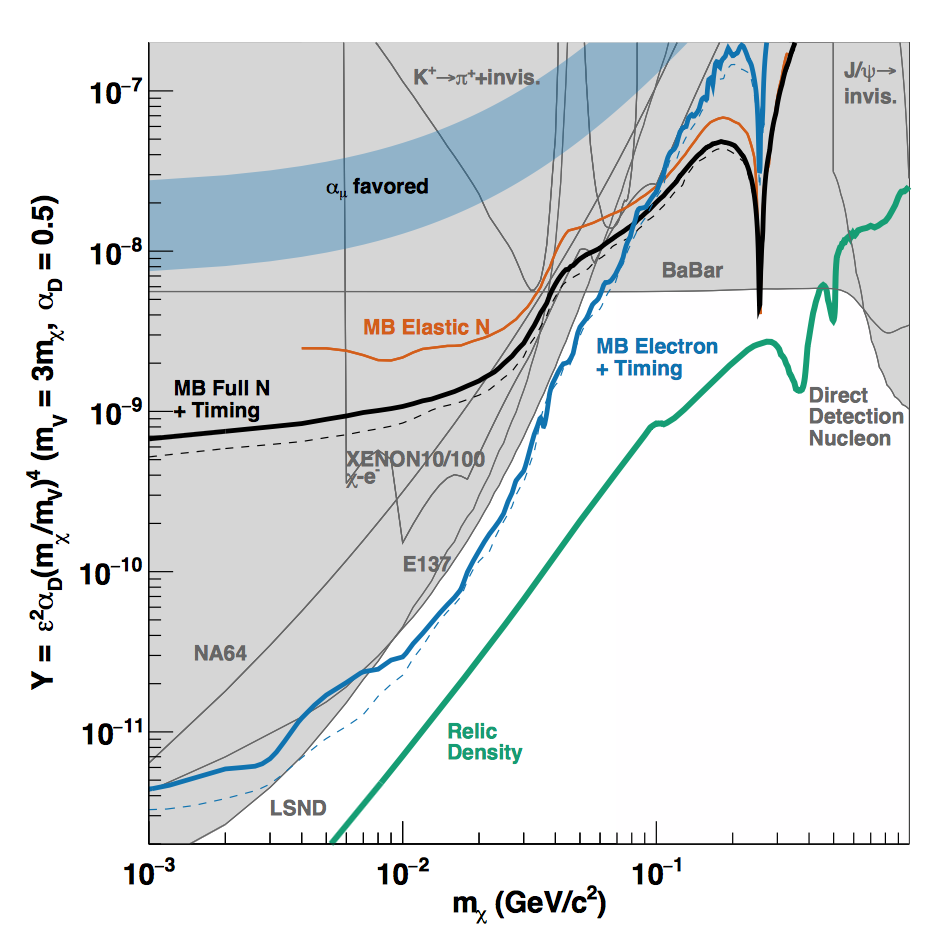
\includegraphics[width=0.7\textwidth,height=3.5in]{graphics/MB-plot.png}
\end{dunefigure}
%%%%%%%%%%%%%%%%%%%%%%%%%%

More scenarios for Dark Matter detection will become accessible for DUNE, due to its improved sensitivity
using LarTPC technology, and the large FD volume, These scenarios include boosted dark matter, 
produced in models with 
a multi-particle dark sector. Sensitivities of such scenarios will be 
examined further in Chapter~\ref{ch:bsm} of this volume.


\subsection{Sterile neutrino search}
 Experimental results in tension with the three-neutrino-flavor paradigm, which may be interpreted
 as mixing between the known active neutrinos and one or more sterile states, have led to a rich
 and diverse program of searches for oscillations into sterile neutrinos. DUNE will be sensitive over a
 broad range of values of the sterile neutrino mass splitting by looking for disappearance of charged
 current (CC) and NC interactions over the long distance separating the near and far detectors,
 as well as over the short baseline of the ND. 
%The ND provides most of the sensitivity at values
% larger than 1 eV2, which where the LSND best-fit and the regions still allowed by fits to global
% data reside. The combination of the intense Long-Baseline Neutrino Facility (LBNF) beam, and a
% highly-capable ND provide DUNE with strong sensitivity in those regions, specifically in probing
% sterile-driven electron neutrino appearance and/or tau neutrino appearance (along with associated
% muon neutrino disappearance). The combination of high-resolution ND components, capable of
% high-efficiency particle ID, combined with a precise muon monitor system for the LBNF beam
% would further enhance this sensitivity.

%There are several categories whose signals would manifest themselves as deviations from the known measured ``standard model'' of neutrinos~\cite{Asaka:2005an,ASAKA200517}. It is clear that any search for deviations of this model is limited by our knowledge of the standard parameters and will always be so. 
The present lead in the search for sterile neutrinos, those which couple to standard neutrinos but not to the weak interaction, comes from disappearance experiments such as muon-neutrino accelerators and reactor anti-neutrino experiments, where unitarity is a necessary assumption. All the most precise measurements of the standard oscillation parameters have been made by disappearance experiments as shown in the left panel of Figure~\ref{fig:disappearance}. The \dword{lsnd} and \miniboone anomalies are expected to be elucidated by \microboone due to its unprecedented event reconstruction capabilities. After the recent measurement from MINOS+ and IceCube are combined with unitarity constraints (see e.g.~\cite{Parke:2015goa}), most of the favored parameter space to explain \dword{lsnd} and \miniboone, with a sterile neutrino, is now disfavored as shown in the right panel of Figure~\ref{fig:disappearance}. Addressing the apparent excess of electron events appearing in the muon-neutrino beam at \miniboone and \dword{lsnd} is also the main goal for the future SBN program at Fermilab, using for the first time near and far detectors with the same technology for this study. Furthermore  in the next years conclusive results will become available from very short baseline 
reactor experiments, which measure the rate of inverse beta decay 
as function of length to the reactor core. These aim to see
small modulations as function of distance, which could be caused
by sterile neutrinos. However given the ensemble of 
all present data so far, if the anomalies survive it seems to 
indicate that a (or a few) 'standard' sterile neutrino(s) 
hypothesis does not fit the data and the explanation may turn
out to be much more complex, in which case certainly the capabilities of the DUNE experiment will play an important role 
in unraveling the exact nature of the new phenomenon.


\begin{dunefigure}[Exclusion limits for muon neutrino disappearance to sterile species in a 3+1 model]{fig:disappearance}
{Left panel: Comparison of present exclusion limits from various experiments obtained through searches for disappearance of muon neutrinos into sterile species assuming a 3+1 model.  The Gariazzo et al. region represents a global fit to neutrino oscillation data~\cite{Gariazzo_2015}. 
    Right panel: The combined results of the disappearance measurements from \dword{minosplus}, \dword{dayabay}, and \dword{bugey}, compared to the appearance measurements from \dword{lsnd} and \miniboone.}
    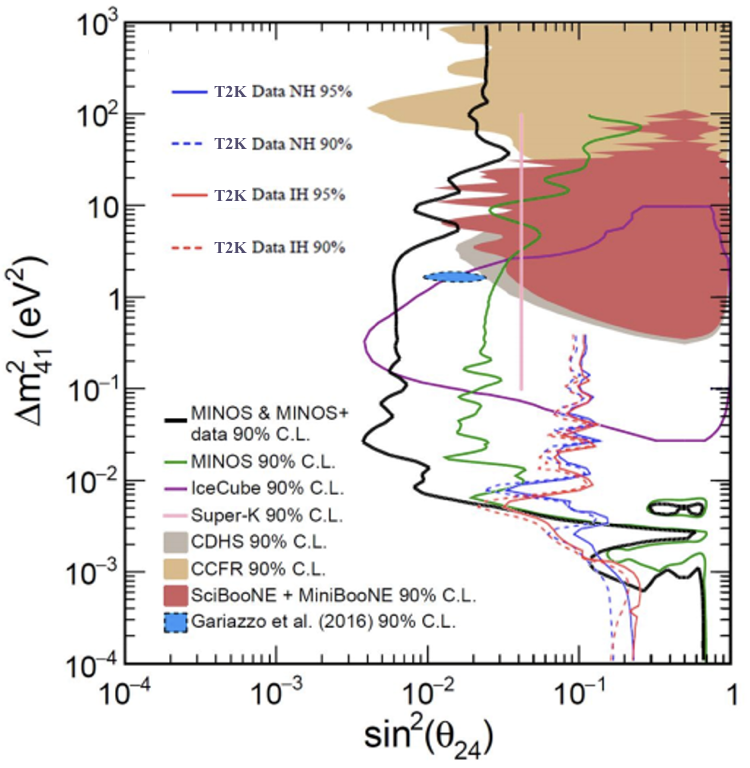
\includegraphics[height=3.5in,width=0.43\textwidth]{graphics/disappearance}
    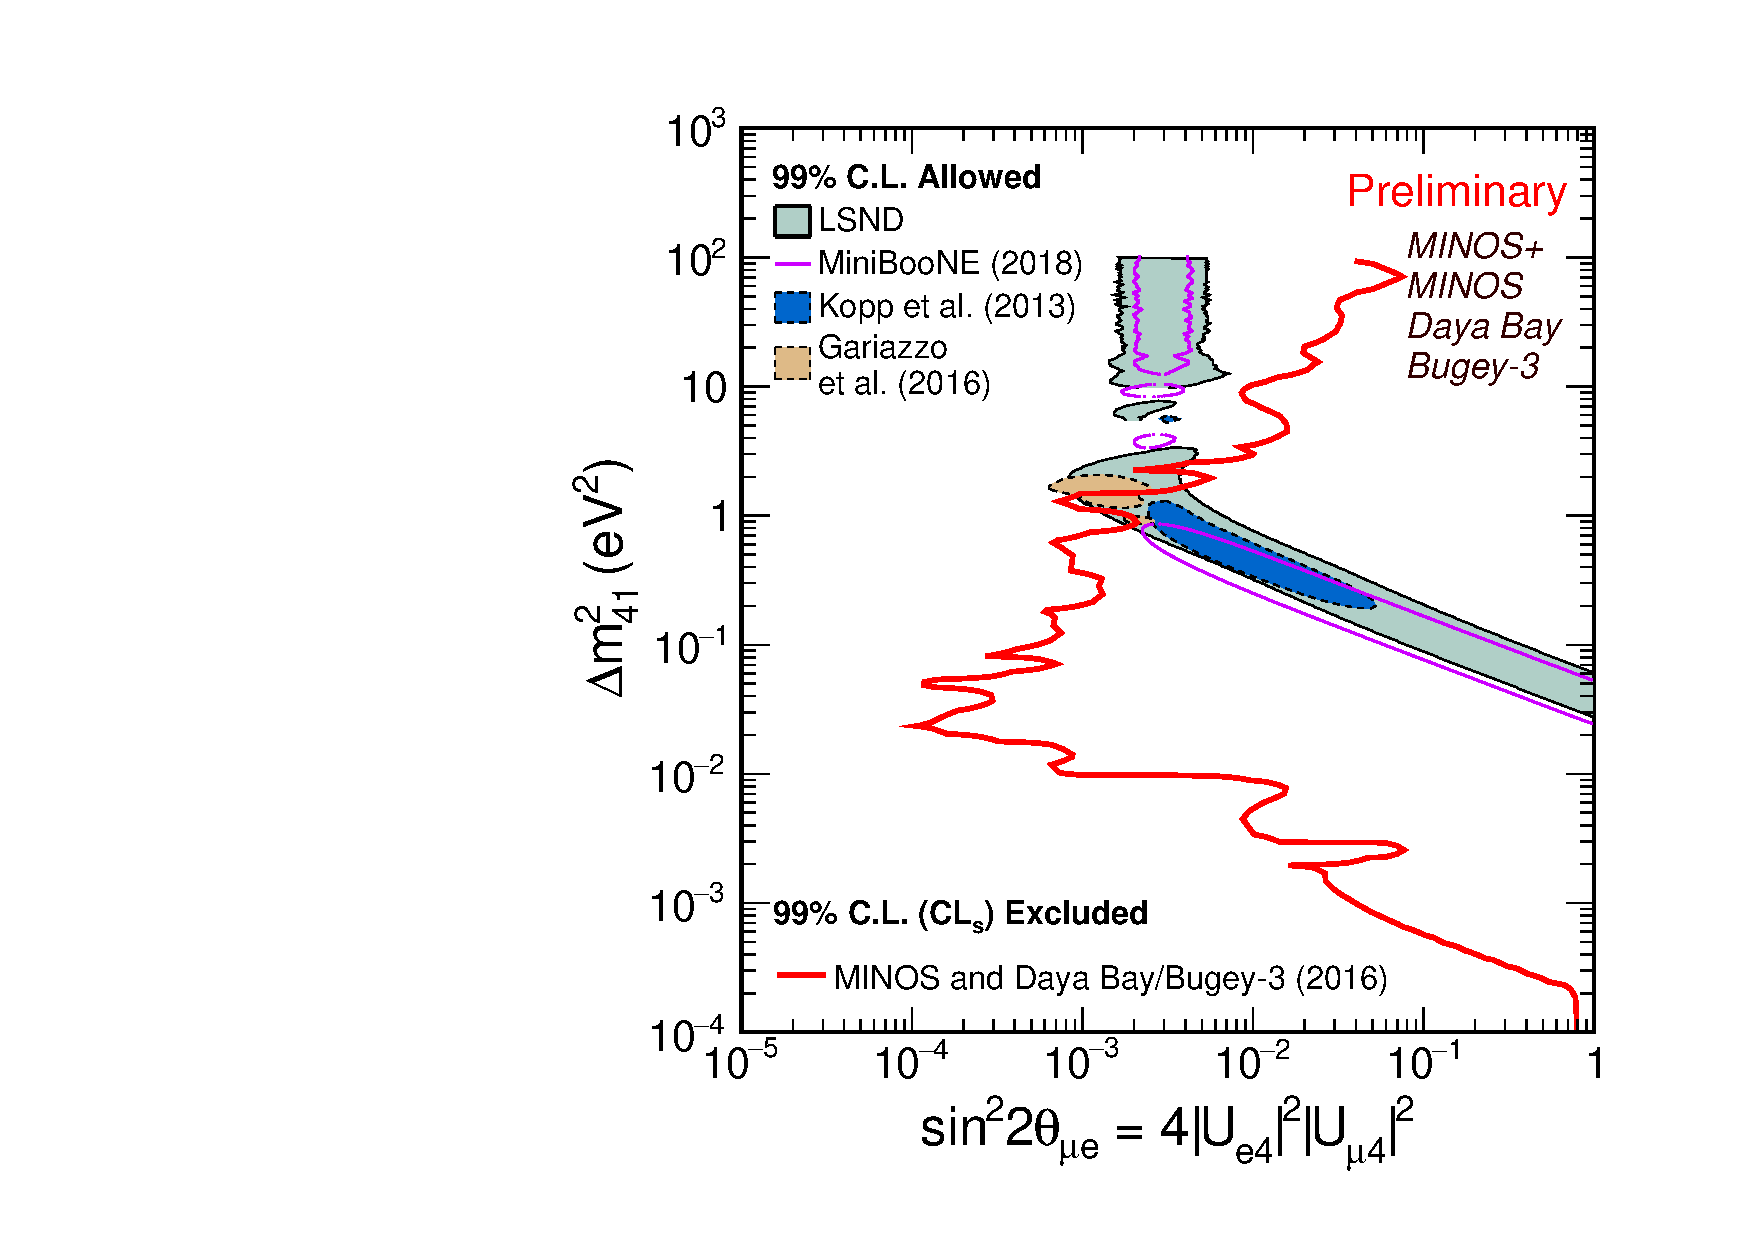
\includegraphics[height=3.7in,width=0.47\textwidth]{graphics/ComboLimit99_prelim.pdf}
\end{dunefigure}


\subsection{Neutrino tridents}
 Neutrino trident production is a rare weak process in which a neutrino, scattering off the Coulomb
 field of a heavy nucleus, generates a pair of charged leptons. The typical final state of a neutrino
 trident interaction contains two leptons of opposite charge. Measurements of muonic neutrino
 tridents were carried out at the CHARM-II, CCFR, and NuTeV experiments, and yielded results
 consistent with Standard Model predictions, but those measurements leave ample room for 
 potential searches for New Physics. As an example, a class of models that modify the trident cross
 section are those that contain an additional neutral gauge boson, $Z_0'$, 
 that couples to neutrinos and charged leptons. This $Z_0'$
 boson can be introduced by gauging an anomaly-free global symmetry
of the Standard Model, with a particular interesting case realized by gauging L$_{\mu}$--L$_{\tau}$. Such a $Z_0'$
 is not very tightly constrained and could address the observed discrepancy between the Standard
Model prediction and measurements of the anomalous magnetic moment of the muon, (g--2)$_{\mu}$
 The DUNE ND offers an excellent environment to generate a sizable number of trident events,
  offering very promising prospects to both improve the above measurements, and to
 look for an excess of events above the Standard Model (SM) prediction, which would be an 
  indication of new physics. 
  
  %In particular, DUNE can potentially discover or rule out the complete
 %parameter space allowed for the ZÕ0 to explain the g-2 anomaly. 
  Another category of BSM Physics
 models that can be probed through neutrino trident measurements are dark neutrino sectors. In
 these scenarios, SM neutrinos mix with heavier SM singlet fermions (dark neutrinos) with their
 own new interactions. Due to this mixing, neutrinos inherit some of this new interaction and may
 up-scatter to dark neutrinos. These heavy states in turn decay back to SM fermions, giving rise
 to trident signatures. These scenarios can explain the smallness of neutrino masses and possibly
 the MiniBooNE low energy excess of events, discussed above.
 % Reconstruction of neutrino trident events would be
% strongly enhanced by a gaseous argon component in the DUNE ND, and the inclusion of a magnetic field could dramatically improve background removal capability by providing sign-selection
% of the opposite charge leptons in the final state of the trident interaction.

\subsection{Heavy neutral leptons}
 The DUNE ND can be used to search topologies of rare event interactions and decays that originate
 from very weakly-interacting long-lived particles, including heavy neutral leptons -- right-handed
 partners of the active neutrinos, vector, scalar, or axion portals to the hidden sector, and light
 supersymmetric particles. The high intensity of the NuMI source and the capability of production
 of charm mesons in the beam allow accessing a wide variety of lightweight long-lived, exotic,
 particles. Competitive sensitivity is expected for the case of searches for decay-in-flight of sub-GeV
 particles that are also candidates for dark matter, and may provide an explanation for leptogenesis
 in the case of charge-parity symmetry violation (CPV) indications. DUNE would probe the lighter
 particles of their hidden sector, which can only decay in SM particles in the form of pairs like $e^+e^-$ ,
 $\mu^+\mu^-$ , qq. The parameter space explored by the DUNE ND extends to the cosmologically relevant
region that is complementary to the LHC heavy-mass dark-matter searches through missing energy
 and mono-jets. 
%The DUNE ND can therefore compete with, and complement, the measurements
% to be carried out by the SHiP experiment, expected to be starting operations at CERN on a time
% scale similar to DUNEÕs, as well as extend or confirm results from searches presently being carried
% out at MicroBooNE, or in the near future with the SBN program.

A recent study on the present limits  and capabilities with future experiments for covering the coupling-mass phase space 
is shown in Figure \ref{fig:bc7_pbc_2}, taken from \cite{Beacham:2019nyx}. These future prospects  cover the experiments, such as the SHiP experiment
 proposed
through the  physics beyond collider study cover the period of the next 10-15 years, hence the same period as for DUNE. The FCC 
curve corresponds to a study much further in the future.

%--------------------------------
\begin{dunefigure}[Sensitivities to heavy neutral leptons]{fig:bc7_pbc_2}
    {Sensitivity to Heavy Neutral Leptons with coupling to the second lepton generation only.
    Current bounds (filled areas) and 10-15 years prospects for PBC projects (SHiP, MATHUSLA200, CODEX-b and FASER2) (dotted and solid lines).
    Projections for the LBNE near detector with $5 \times 10^{21}$ pot and  FCC-ee with $10^{12}$ $Z^0$
    decays are also shown.}
  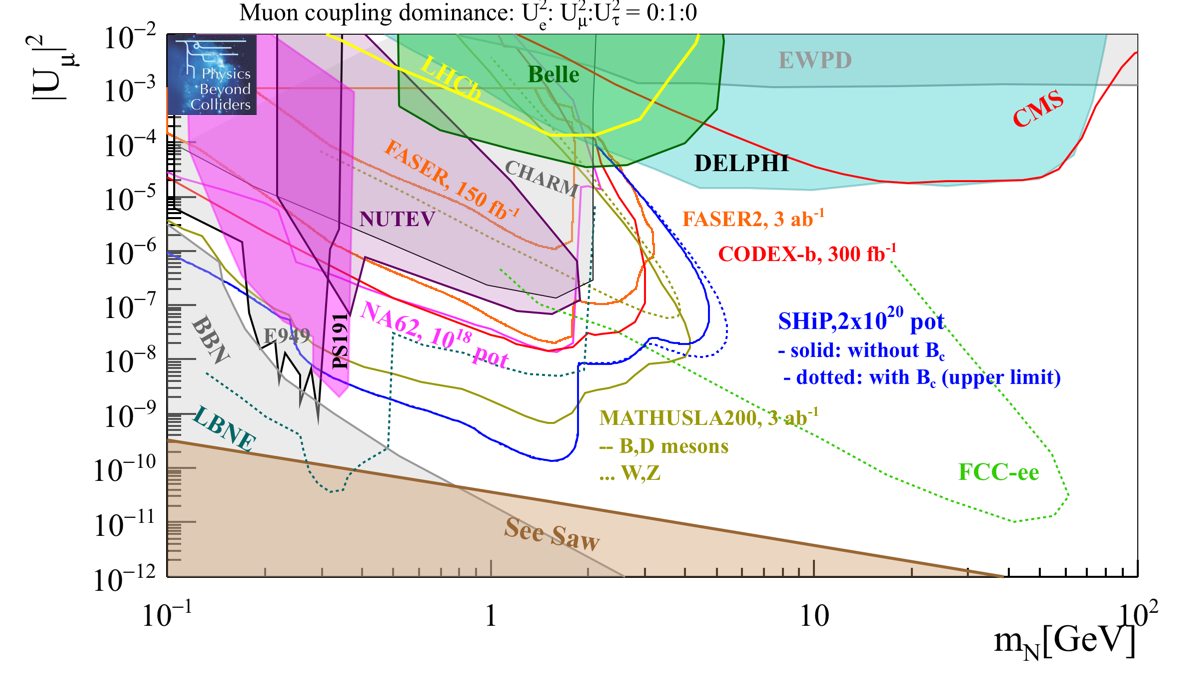
\includegraphics[width=0.8\linewidth]{HNL_bc7_pbc_2.png}
\end{dunefigure}
%--------------------------------

%Comment on other A0 etc?

%30 6.0.5 Non-standard Neutrino Interactions
%31 While the role of ND in this measurement is less significant, DUNE can also search for deviations
%32 from the Pontecorvo-Maki-Nakagawa-Sakata (PMNS) neutrino mixing paradigm arising due to
%33 nonstandard interactionss (NSIs), in particular those occurring at neutrino production, which
%34 would leave subtle imprints in the neutrino flux. Sensitivity to these effects would require a
%35 very well characterized flux for it to be competitive with probes of the same phenomenon in
%36 coherent electron neutrino scattering experiments. Further, the more common search for NSI
%37 affecting neutrino propagation through the Earth benefits from constraints on cross section and
%38 flux provided by a highly-capable ND in the same way as the CPV probe would. If the DUNE
%39 data are consistent with standard oscillations for three massive neutrinos, interaction effects of
%order 0.1 GF can be ruled 1 out at DUNE. DUNE could improve current constraints on e and ?e
%2 by a factor 2 to 5.